% vim: ts=2:sw=2:tw=80:et
\thispagestyle{fancy}
\pagestyle{fancy}

This manual describes the use and operation of Arbwave, the arbitrary waveform
experimental control program.

\section{What is Arbwave?\index{What is Arbwave?}}
\subsection{Background}
Atomic physics experiments typically involve various voltages, currents,
magnetic fields, laser fields, and mechanical devices that must be manipulated
and altered according to very precise relative timing relationships.  It is
necessary to use hardware and software that provides for coordinating these
tight timing relationships.  The extent to which software and hardware are
able to present these timing relationships to a user in a succinct and
consistent fashion directly determines how well a configuration can be
tailored to the specific experimental situation.

\subsection{Open Source Software}
Arbwave is part of an effort from the Air Force Research Laboratory
(\acro{AFRL}) Cold-Atoms group to develop a platform suitable for typical atomic
physics experiments.  One of the goals of this effort is to provide a simple,
consistent view and control of experimental timing parameters.  This software is
released to the public in the form of an Open Source Software (\acro{OSS})
project.  This is done with the intent and hope that the community in general
can benefit from \acro{AFRL}'s work on Arbwave and to also foster collaboration
for and sharing of special experimental expertise permeating throughout the
scientific community.

\subsection{License/Terms}
This program is free software: you can redistribute it and/or modify it under
the terms of the
\href{https://www.gnu.org/licenses/gpl-3.0.en.html}
{GNU General Public License, version 3}, as published by the Free
Software Foundation.  This program is distributed in the hope that it will be
useful, but \underline{WITHOUT} ANY WARRANTY; \underline{without} even the
implied warranty of MERCHANTABILITY or FITNESS FOR A PARTICULAR PURPOSE.  For
full license requirements with regards to copying, modifying, and distributing,
see the full text of the GPLv3 license.  For convenience, some portions of the
license are copied here.  You should have received a copy of the GNU General
Public License along with this program.  If not, see
\url{https://www.gnu.org/licenses/}.


\subsubsection{Rights and Responsibilities}
When a program, such as Arbwave, is licensed under the GNU General Public
License (the \acro{GPL}):
\begin{itemize}[noitemsep,partopsep=0em,parsep=0em]
\item You have the right to use the program for any purpose.
\item You have the right to modify the program and have access to the source codes.
\item You have the right to copy and distribute the program.
\item You have the right to improve the program, and release your own versions.
\end{itemize}

In return for these rights, you have some responsibilities if you distribute a
\acro{GPL}-licensed program, responsibilities that are designed to protect your
freedoms and the freedoms of others:
\begin{itemize}[noitemsep,partopsep=0em,parsep=0em]
\item You must provide a copy of the \acro{GPL} with the program, so that
      recipients are aware of their rights under the license;
\item You must include the source code or make the source code freely available;
\item If you modify the code and distribute the modified version, you must
      license your modifications available under the \acro{GPL} (or a compatible
      license);
\item You may not restrict the licensing of the program beyond the terms of the
      \acro{GPL} (i.e. you may not turn a \acro{GPL}-licensed program into a
      proprietary product).
\end{itemize}
For more information, see \url{https://www.gnu.org/licenses/}.


\subsubsection{Disclaimer of Warranty}
As per the \href{https://www.gnu.org/licenses/gpl-3.0.en.html}{GPLv3 license},
Section 15, no warranty of this software or associated documentation is
given\cite{gplv3}:
\begin{quote}
THERE IS NO WARRANTY FOR THE PROGRAM, TO THE EXTENT PERMITTED BY APPLICABLE LAW.
EXCEPT WHEN OTHERWISE STATED IN WRITING THE COPYRIGHT HOLDERS AND/OR OTHER
PARTIES PROVIDE THE PROGRAM “AS IS” WITHOUT WARRANTY OF ANY KIND, EITHER
EXPRESSED OR IMPLIED, INCLUDING, BUT NOT LIMITED TO, THE IMPLIED WARRANTIES OF
MERCHANTABILITY AND FITNESS FOR A PARTICULAR PURPOSE. THE ENTIRE RISK AS TO THE
QUALITY AND PERFORMANCE OF THE PROGRAM IS WITH YOU. SHOULD THE PROGRAM PROVE
DEFECTIVE, YOU ASSUME THE COST OF ALL NECESSARY SERVICING, REPAIR OR CORRECTION.
\end{quote}

Furthermore, in no fashion does this release guarantee completeness of the
documentation.

\subsubsection{Limitation of Liability}
As per the \href{https://www.gnu.org/licenses/gpl-3.0.en.html}{GPLv3 license},
Section 16, this software and associated documentation is released with limited
liability\cite{gplv3}:
\begin{quote}
IN NO EVENT UNLESS REQUIRED BY APPLICABLE LAW OR AGREED TO IN WRITING WILL ANY
COPYRIGHT HOLDER, OR ANY OTHER PARTY WHO MODIFIES AND/OR CONVEYS THE PROGRAM AS
PERMITTED ABOVE, BE LIABLE TO YOU FOR DAMAGES, INCLUDING ANY GENERAL, SPECIAL,
INCIDENTAL OR CONSEQUENTIAL DAMAGES ARISING OUT OF THE USE OR INABILITY TO USE
THE PROGRAM (INCLUDING BUT NOT LIMITED TO LOSS OF DATA OR DATA BEING RENDERED
INACCURATE OR LOSSES SUSTAINED BY YOU OR THIRD PARTIES OR A FAILURE OF THE
PROGRAM TO OPERATE WITH ANY OTHER PROGRAMS), EVEN IF SUCH HOLDER OR OTHER PARTY
HAS BEEN ADVISED OF THE POSSIBILITY OF SUCH DAMAGES.
\end{quote}


\subsection{What can Arbwave do?}
Arbwave provides a means for a user to clearly coordinate groups of transitions
for various control signals that can be used to run a complicated experimental
timing sequence.  In Arbwave, a series of channels are defined where each
channel represents some control signal used to supervise an experimental
parameter such as voltage, current, magnetic field, etc.  Using the
information of the defined channels, Arbwave allows one to coordinate
hierarchical sets of transitions for each of those channels.  Arbwave also
graphically represents each of the signal transitions as complete waveforms
where the time for each transition is accurately shown.  Furthermore, Arbwave
facilitates execution of these waveforms in various operation patterns, such
as control-variable nested loop iteration and multi-variable optimization.
Finally, user scripting, via Python, can be inserted into the execution to
customize a particular experimental procedure, customize an optimization
procedure, and hook into various external data recorders processors.


\section{Design Approach}

\begin{figure}[ht!]
  \centerline{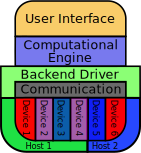
\includegraphics[width=.4\textwidth]{figures/design-layout}}
  \caption[Arbwave design architecture]{
    Abstract view of Arbwave design architecture.  Arbwave is divided into
    abstracted layers to separate implementation details.
  }
  \label{fig:intro:design}
\end{figure}

As shown in Fig.~\ref{fig:intro:design}, Arbwave is designed as a layered
operation platform.  Each layer represents a sent of tasks or compartments of
computational requirements.  The interfaces between each layer are abstracted
such that only hardware-agnostic, generic interfaces are used.  The consistent
interfaces and abstraction concepts allow interaction between the layers without
strict need to understand the internals of the other layers.

Furthermore, this abstracted approach allows various layers and components of
Arbwave to be developed and extended without affecting the general operation of
the entire platform.  For example, since the hardware layer is abstracted away
from the computational engine and user interface of Arbwave, it was possible to
insert a near seamless communication layer that allows parts of the accessible
hardware to be provided by a remote connection.  Thus, as indicated in the lower
portion of Fig.~\ref{fig:intro:design}, several devices from various hosts can
be aggregated together for common control for a single experiment.
Additionally, because of this abstraction, it is possible to add support for new
hardware without disruption to the user interface and computational engine
layers: one must only implement the interfaces that Arbwave requires.


\subsection{Supported Hardware\index{Supported Hardware}}\label{sec:hardware}

Because the design of Arbwave abstracts the hardware support, adding new hardware does
not impact the normal functions of the platform.  It is possible, therefore, to
support a range of hardware and hardware drivers.  Tab.~\ref{tab:drivers} shows
the various hardware drivers and related devices for which the Arbwave backend
layer implements the required driver interfaces.

\begin{table}[ht!]
\begin{center}
  \begin{tabular}{|l|c|p{6.5cm}|p{2cm}|r|}
    \hline
    \textbf{\large Manufacturer} &
    \textbf{\large Model} &
    \textbf{\large Description} &
    \textbf{\large Supported Driver(s)} &
    \textbf{\large Platform(s)} \\
    \hline
    \hline
    NI          &    *      & Various--see Tab.~\ref{tab:daqmx}& \acro{DAQmx}
                & Windows \\
    Various     &    *      & Various third-party devices on Linux & \acro{COMEDI}
                & Linux \\
    Viewpoint   & DIO-64    & Digital input/output, 64-channel & DIO64
                & Windows \\
    Marvin Test & GX164x    & 16-bit Analog output, 64-channel & GxAo
                & Linux, Windows \footnotemark \\
    Marvin Test & GX3500    & FPGA based digital output, 120-channel & GxFpga
                & Linux, Windows \footnotemark \\
    N/A         & DDSTiming & AFRL DDS/Timing Cape for Beaglebone black & N/A
                & N/A \\
    \hline
  \end{tabular}
  \label{tab:drivers}
  \caption{Supported Hardware Drivers}
\end{center}
\end{table}
\footnotetext{Development still in progress}
\footnotetext{Windows support not yet tested}


\subsubsection{National Instruments: \acro{DAQmx}}
Arbwave requires the knowledge of signal connections that are possible
with the various \acro{DAQmx} hardware.  As of yet, this information is only
known to be available via the NI-MAX Windows software from National
Instruments--no known documentation of these valid routes exists and no
programming interface to the \acro{DAQmx} c-library appears to give this
information.

Arbwave's use of \acro{DAQmx} generally provides support to most
analog and digital output hardware supported by \acro{DAQmx}.  In spite of this,
a small amount of information pertaining to direct signal routing
is needed to satisfy Arbwave coordinated timing requirements.
Tab.~\ref{tab:daqmx} shows a list of \acro{DAQmx} devices for which routing
information has been already included as of the date specified.

\begin{table}[ht!]
\centering
  \begin{tabular}{|l|cccc|}
    \hline
    Board Label & Bit-depth & AI & AO & DIO\footnotemark \\
    \hline
    \hline
    PCI-6070E & 12 & 16 & 2 & 0  \\
    PXI-6030E & 16 & 16 & 2 & 0  \\
    PCI-6220  & 16 & 16 & 0 & 8  \\
    PCI-6221  & 16 & 16 & 2 & 8  \\
    PXI-6224  & 16 & 32 & 0 & 32 \\
    PXI-6225  & 16 & 80 & 2 & 8  \\
    PCI-6225  & 16 & 80 & 2 & 8  \\
    PCI-6229  & 16 & 32 & 4 & 32 \\
    PCI-6251  & 16 & 16 & 2 & 8  \\
    PXI-6251  & 16 & 16 & 2 & 8  \\
    PXIE-6251 & 16 & 16 & 2 & 8  \\
    PCI-6254  & 16 & 32 & 0 & 32 \\
    PCI-6259  & 16 & 32 & 4 & 32 \\
    PCI-6534  & xx &  0 & 0 & 32 \\
    PCI-6733  & 16 &  0 & 8 & 0  \\
    PXI-6733  & 16 &  0 & 8 & 0  \\
    PCI-6713  & 12 &  0 & 8 & 0  \\
    PCI-6723  & 12 &  0 & 32& 0  \\
    \hline
  \end{tabular}
  \caption{
    \label{tab:daqmx}
    \acro{DAQmx} hardware with routing information included as of 13~Oct~2017.
  }
\end{table}

In order to use additional \acro{DAQmx} devices with Arbwave, it is
necessary to first add this routing information (gathered from NI-MAX) to the
Arbwave.backend.drivers.nidaqmx.routes sub-package found in the\\
\noindent \texttt{python/arbwave/backend/drivers/nidaqmx/routes.py} file.

\footnotetext{Only clocked or correlated digital (DIO) lines which are useful for
Arbwave timing are indicated}
